\documentclass[compress]{beamer}

\mode<presentation>
{
	\usetheme{Singapore}
	\usecolortheme{lily}

	\setbeamertemplate{footline}[frame number]
	\setbeamertemplate{navigation symbols}{}

	% \usecolortheme{beetle} % una mica millor (blanc sobre gris)
	% \usecolortheme{dolphin}
	% \usecolortheme{dove} % (gris i negre sobre blanc), molt simple
	% \usecolortheme{fly}
	% \usecolortheme{lily} % me gusta
	% \usecolortheme{rose}
	% \usecolortheme{seagull}

	% \usetheme{marko}
}

\usepackage{graphicx}
\usepackage{booktabs}
\usepackage{media9}
% \usepackage{animate}
\usepackage[amssymb]{SIunits}
\usepackage{listings}
\lstloadlanguages{VHDL}
	% \lstset
	% {
	% 	language=Matlab, %-> choose the language of the code
	% 	basicstyle=\scriptsize,% -> the size of the fonts used for the code
	% 	numbers=left,% -> where to put the line-numbers
	% 	numberstyle=\tiny,% -> size of the fonts used for the line-numbers
	% 	stepnumber=1,% -> the step between two line-numbers.
	% 	numbersep=15pt,% -> how far the line-numbers are from the code
	% 	% backgroundcolor=\color{white},% -> sets background color (needs package)
	% 	showspaces=false,% -> show spaces adding particular underscores
	% 	showstringspaces=false,% -> underline spaces within strings
	% 	showtabs=false,% -> show tabs within strings through particular underscores
	% 	% frame=single,% -> adds a frame around the code
	% 	tabsize=4,% -> sets default tab-size to 2 spaces
	% 	captionpos=t,% -> sets the caption-position to top
	% 	breaklines=true,% -> sets automatic line breaking
	% 	breakatwhitespace=true,% -> automatic breaks happen at whitespace
	% 	keywordstyle=\color{blue},
	% 	linewidth=0.9\textwidth,
	% 	xleftmargin=0.1\textwidth,
	% 	xrightmargin=0\textwidth,
	% 	morekeywords={heaviside,hann,hamming,kaiser,bartlett,blackman,rectwin,triang,chebwin,
	% 	triangulo,pulso,sierra,senos,cuadrados,triangulo1,pulso1,funcz,tdf,hilbert,corr,ezplot},
	% 	extendedchars=true,
	% 	commentstyle=\color[rgb]{0.1,0.5,0.1}
	% }
	% \lstset
	% {
	% 	language=C, %-> choose the language of the code
	% 	basicstyle=\scriptsize,% -> the size of the fonts used for the code
	% 	numbers=left,% -> where to put the line-numbers
	% 	numberstyle=\tiny,% -> size of the fonts used for the line-numbers
	% 	stepnumber=1,% -> the step between two line-numbers.
	% 	numbersep=10pt,% -> how far the line-numbers are from the code
	% 	% backgroundcolor=\color[rgb]{0.95, 0.95, 0.95},% -> sets background color (needs package)
	% 	showspaces=false,% -> show spaces adding particular underscores
	% 	showstringspaces=false,% -> underline spaces within strings
	% 	showtabs=false,% -> show tabs within strings through particular underscores
	% 	% frame=single,% -> adds a frame around the code
	% 	tabsize=2,% -> sets default tab-size to 2 spaces
	% 	captionpos=t,% -> sets the caption-position to top
	% 	breaklines=true,% -> sets automatic line breaking
	% 	breakatwhitespace=true,% -> automatic breaks happen at whitespace
	% 	keywordstyle=\color{blue},
	% 	linewidth=0.95\textwidth,
	% 	xleftmargin=0.05\textwidth,
	% 	xrightmargin=0\textwidth,
	% 	morekeywords={define, byte, millis, map, analogRead, delay, boolean},
	% 	extendedchars=true,
	% 	commentstyle=\color[rgb]{0.1,0.5,0.1}
	% }
	\lstset
	{
		language=, %-> choose the language of the code
		basicstyle={\scriptsize},% -> the size of the fonts used for the code \color[rgb]{0.95,0.95,0.95}
		numbers=left,% -> where to put the line-numbers
		numberstyle={\tiny},% -> size of the fonts used for the line-numbers
		stepnumber=1,% -> the step between two line-numbers.
		numbersep=10pt,% -> how far the line-numbers are from the code
		% backgroundcolor=\color[rgb]{0.95, 0.95, 0.95},% -> sets background color (needs package)
		showspaces=false,% -> show spaces adding particular underscores
		showstringspaces=false,% -> underline spaces within strings
		showtabs=false,% -> show tabs within strings through particular underscores
		% frame=single,% -> adds a frame around the code
		tabsize=2,% -> sets default tab-size to 2 spaces
		captionpos=t,% -> sets the caption-position to top
		breaklines=true,% -> sets automatic line breaking
		breakatwhitespace=true,% -> automatic breaks happen at whitespace
		keywordstyle=\color{blue},
		linewidth=0.95\textwidth,
		xleftmargin=0.05\textwidth,
		xrightmargin=0\textwidth,
		morekeywords={std_logic, std_logic_vector, integer, rising_edge, to_integer, unsigned, to_unsigned},
		extendedchars=true,
		commentstyle=\color[rgb]{0.1,0.5,0.1}
	}

% TEST AREA
	% \AtBeginSection[]
	% {
	%   \begin{frame}
	%     \frametitle{Tabla de contenidos}
	%     \tableofcontents[currentsection]
	%   \end{frame}
	% }
% TEST AREA

% TITLE PAGE
	\title{Detector de nivel de agua y\\comunicaci\'on v\'ia Ethernet con FPGA}
	\author{Marko Peshevski}
	\institute{SDAV, MUESAEI}
	\date{Septiembre - Diciembre, 2016}
% TITLE PAGE

\begin{document}

\begin{frame}[plain]
	\titlepage
\end{frame}

\begin{frame}
    \frametitle{Tabla de contenidos}
    \tableofcontents
\end{frame}

\setcounter{framenumber}{0}
\section{Introducci\'on}
	\subsection{El problema. Objetivo}
		\begin{frame}
			\frametitle{El problema. Objetivo}
				\begin{figure}
					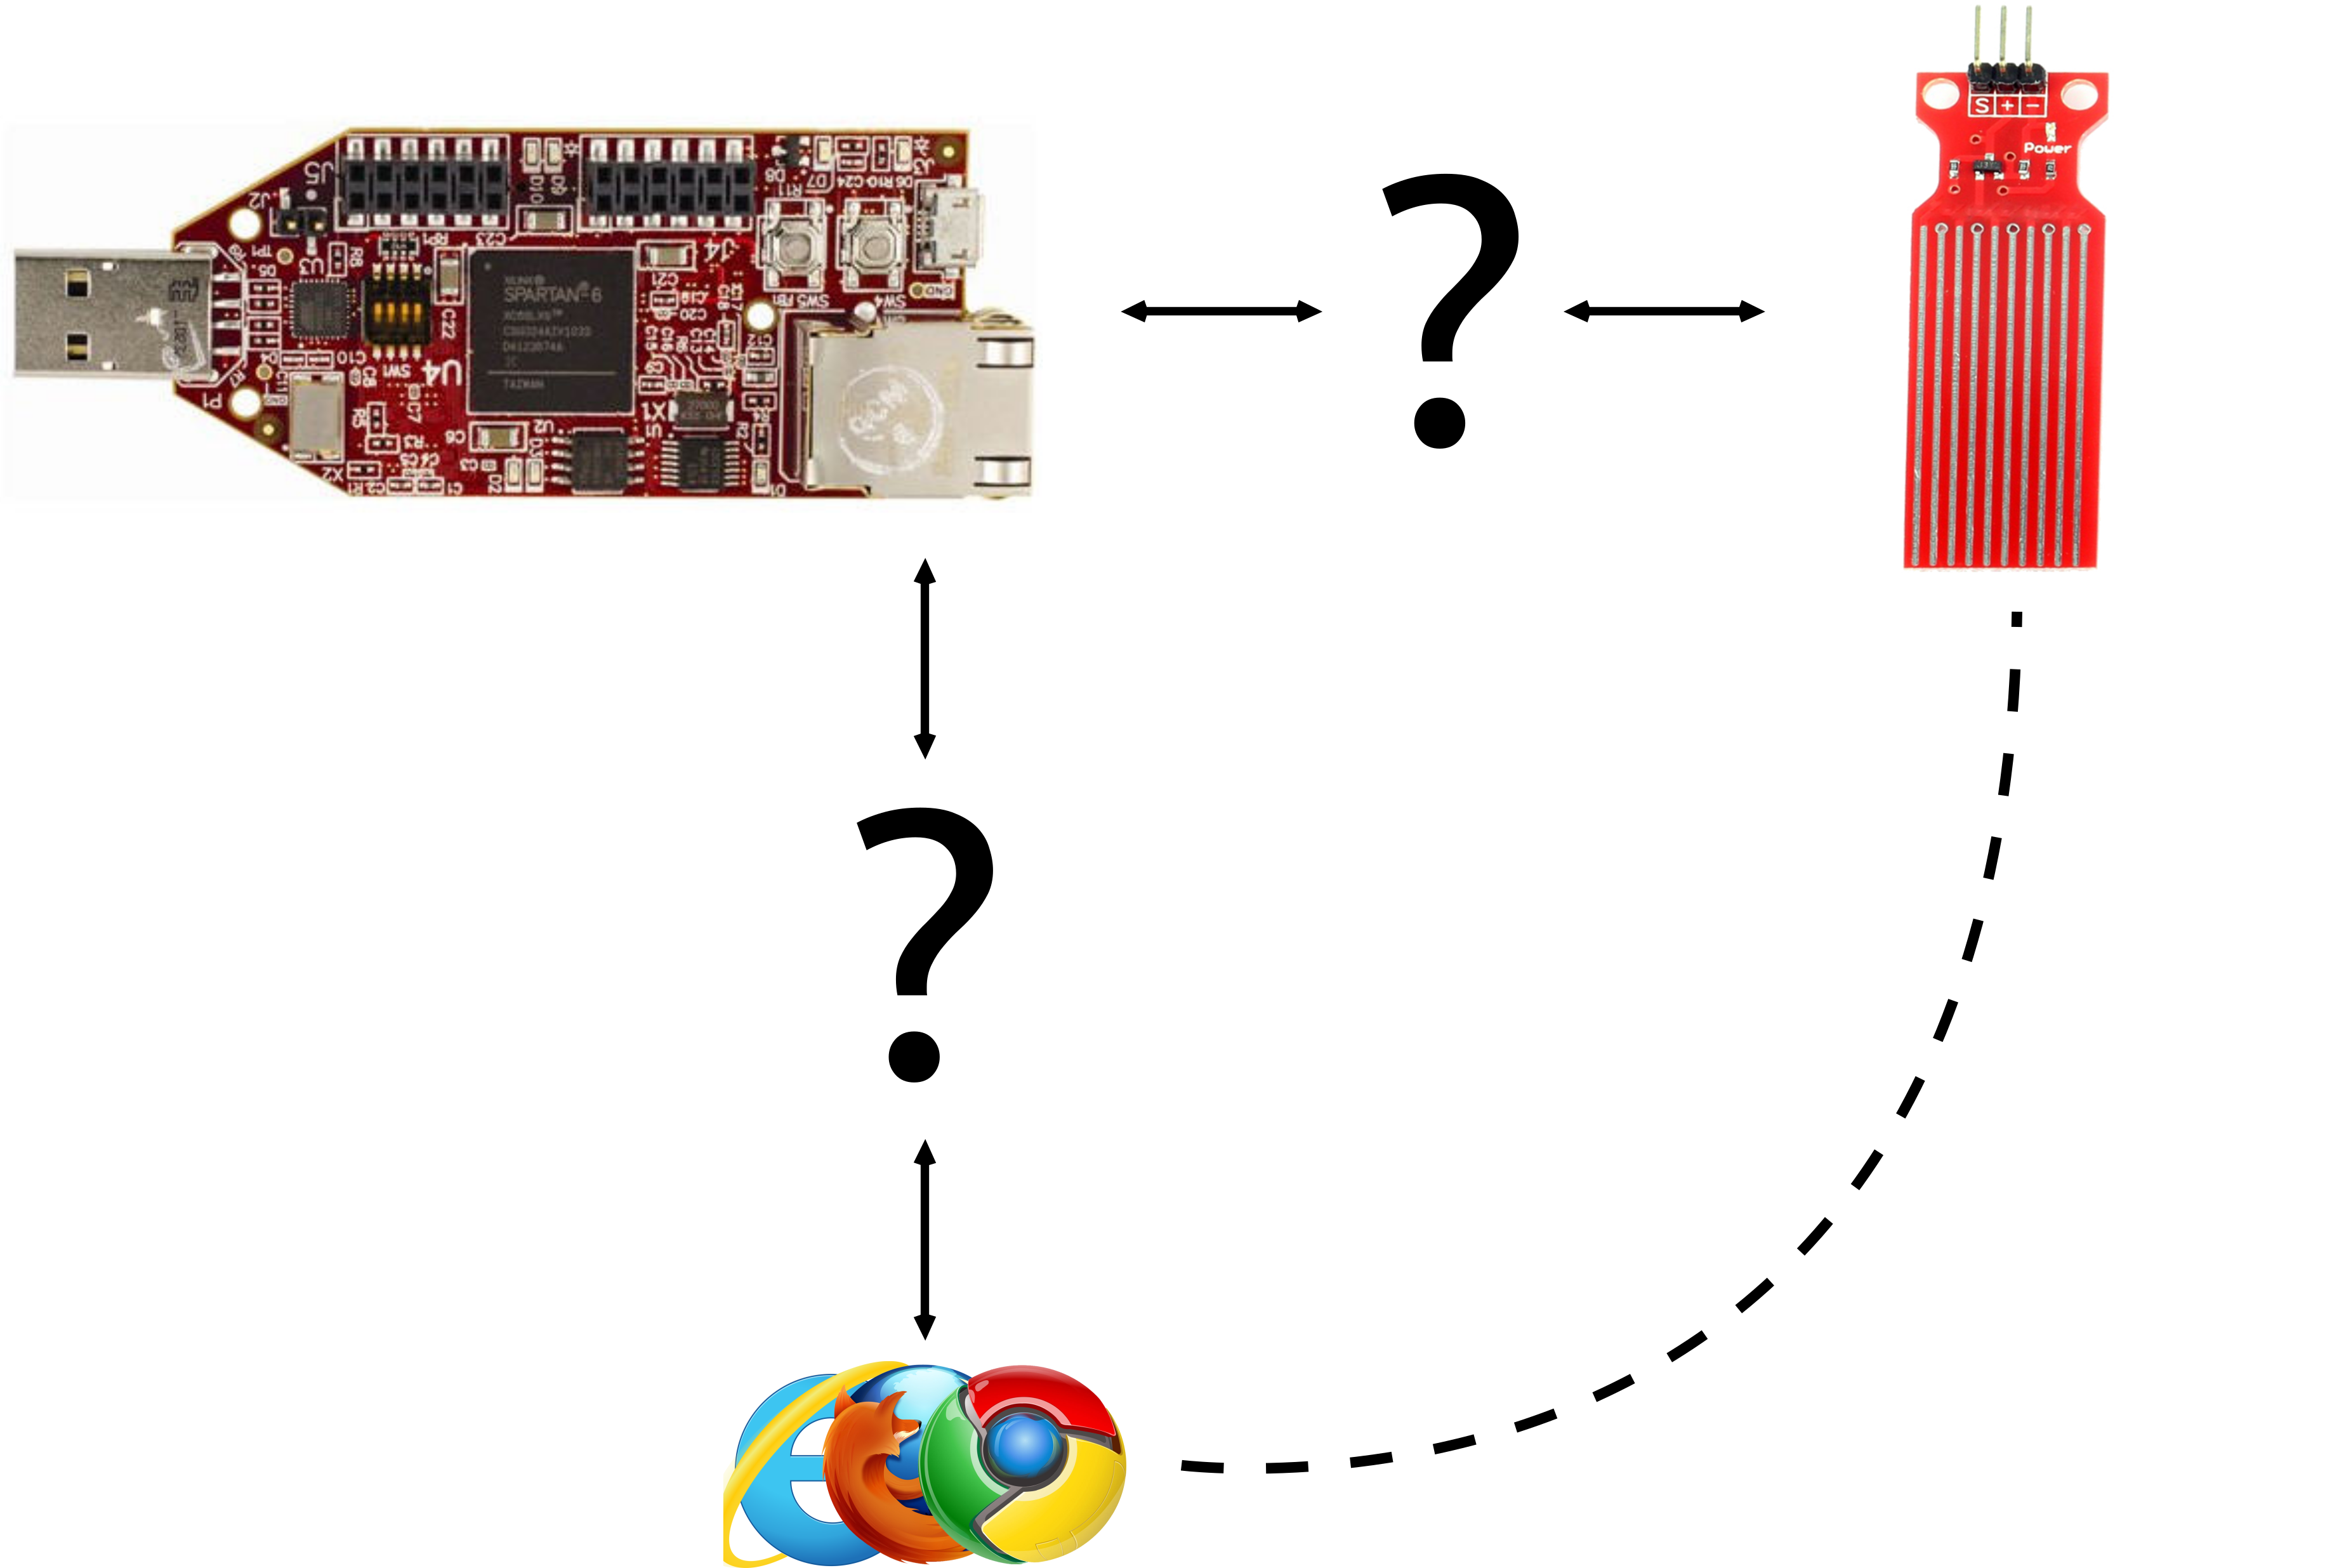
\includegraphics[keepaspectratio = true, width=0.9\textwidth]{figuras/introduccion.png}
				\end{figure}
		\end{frame}

	\subsection{Sensor de nivel de agua}
		\begin{frame}
			\frametitle{Sensor de nivel de agua}
				\begin{itemize}
					\item
					{

						Sensor de muy bajo coste

					}
					\item
					{

						Transistor NPN con resistencia de base variable

					}
				\end{itemize}
				\begin{figure}
					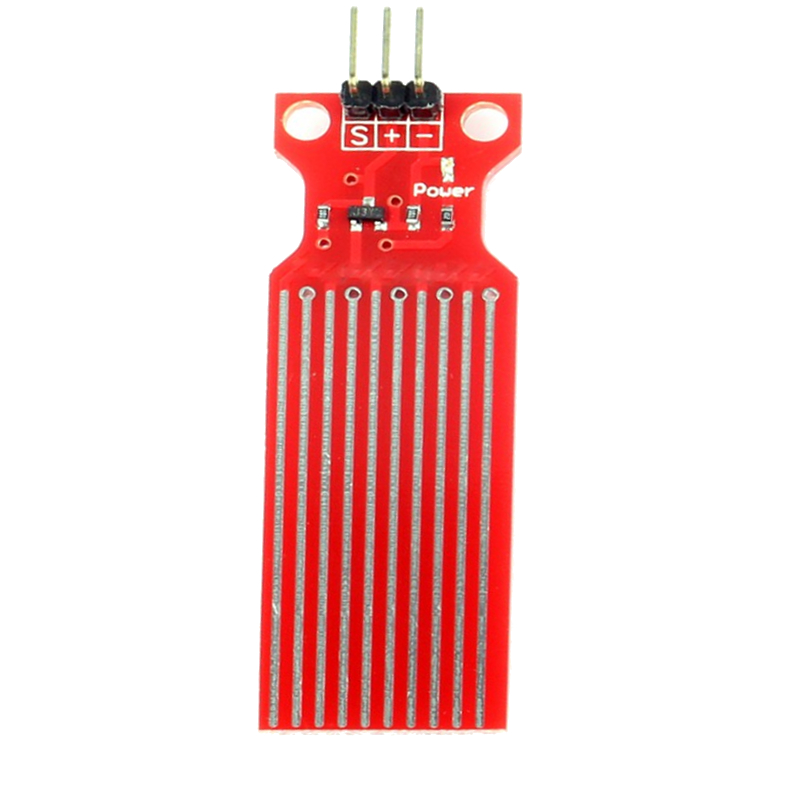
\includegraphics[keepaspectratio = true, totalheight=0.5\textheight]{figuras/sensor.jpg}
					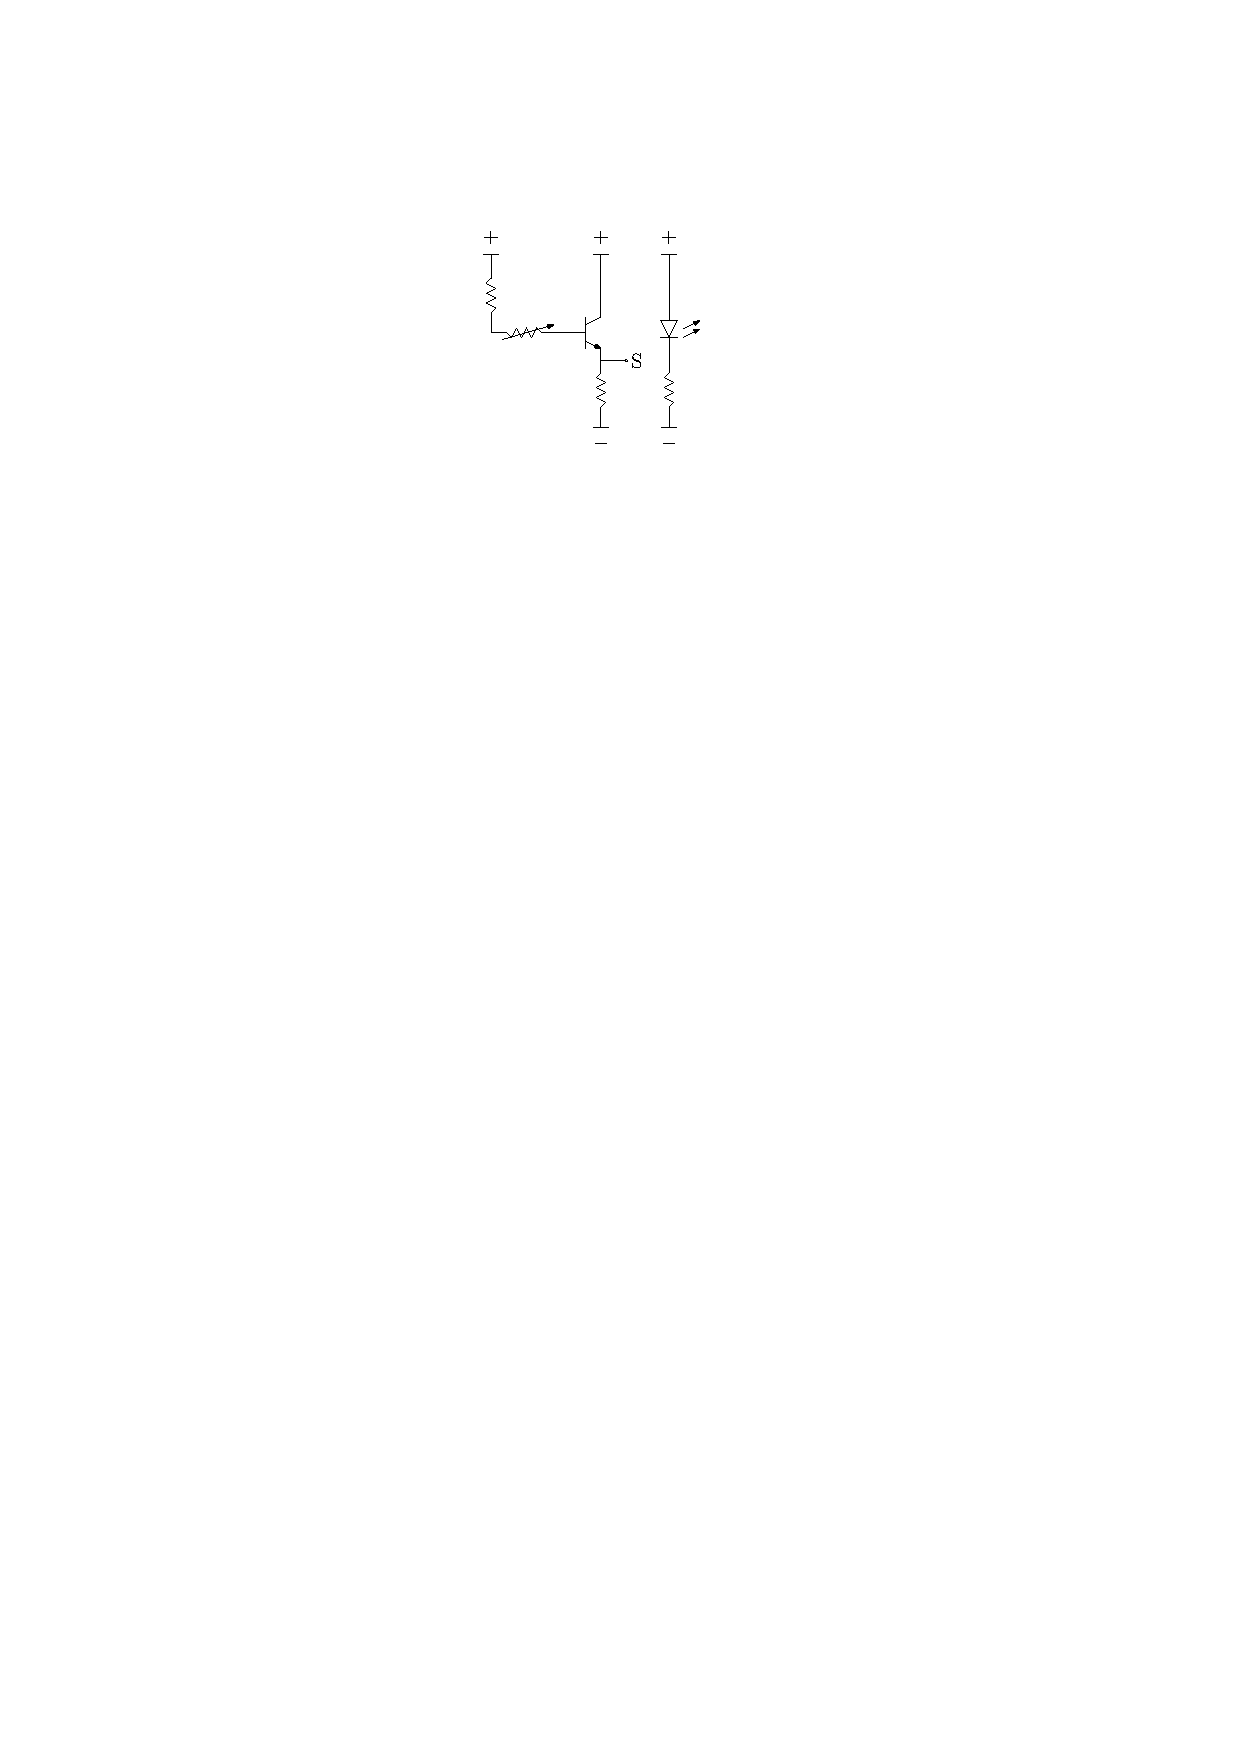
\includegraphics[keepaspectratio = true, totalheight=0.5\textheight]{figuras/circuito.pdf}
				\end{figure}
		\end{frame}

\section{Soluci\'on}
	\subsection{Sensor de agua -- FPGA}
		\begin{frame}
			\frametitle{Soluci\'on}
			\framesubtitle{Sensor de agua -- FPGA}
				\begin{itemize}
					\item
					{

						Conversor anal\'ogico -- digital de 10 bits: MCP3002

					}
					\item
					{

						Comunicaci\'on por SPI, con 3 bits para pedir informaci\'on

					}
					\item
					{

						Parte ya hecha como ejercicio de la asignatura

					}
				\end{itemize}
				\begin{figure}
					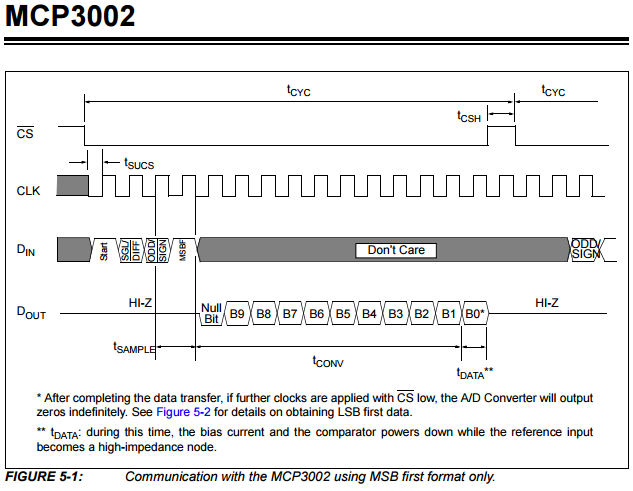
\includegraphics[keepaspectratio = true, totalheight=0.6\textheight]{figuras/adc_spi.png}
				\end{figure}
 		\end{frame}

	\subsection{FPGA -- red}
		\begin{frame}
			\frametitle{Soluci\'on}
			\framesubtitle{FPGA -- red}
				\begin{itemize}
					\item
					{

						Ethernet como interfaz f\'isico para comunicaci\'on TCP/IP con la red

					}
					\item
					{

						Capa de acceso al medio por Ethernet: n\'ucleo IP de Xilinx sobre MicroBlaze (n\'ucleo soft-core corriendo sobre Spartan6)

					}
					\item
					{

						LwIP como librer\'ia TCP/IP para sistemas embebidos, corriendo sobre MicroBlaze

					}
					\item
					{

						Partiendo de un ejemplo de Avnet, se programa un servidor web capaz de comunicarse con un cliente mediante WebSockets

					}
				\end{itemize}

 		\end{frame}

		\begin{frame}
			\frametitle{Soluci\'on}
			\framesubtitle{WebSockets}
				\begin{itemize}
					\item
					{

						Protocolo sobre TCP/IP que permite comunicaci\'on bidireccional as\'incrona entre cliente y servidor

					}
					\item
					{

						Comunicaci\'on muy eficiente, con s\'olo unos pocos bytes adicionales a la informaci\'on a transferir

					}
				\end{itemize}
				\begin{figure}
					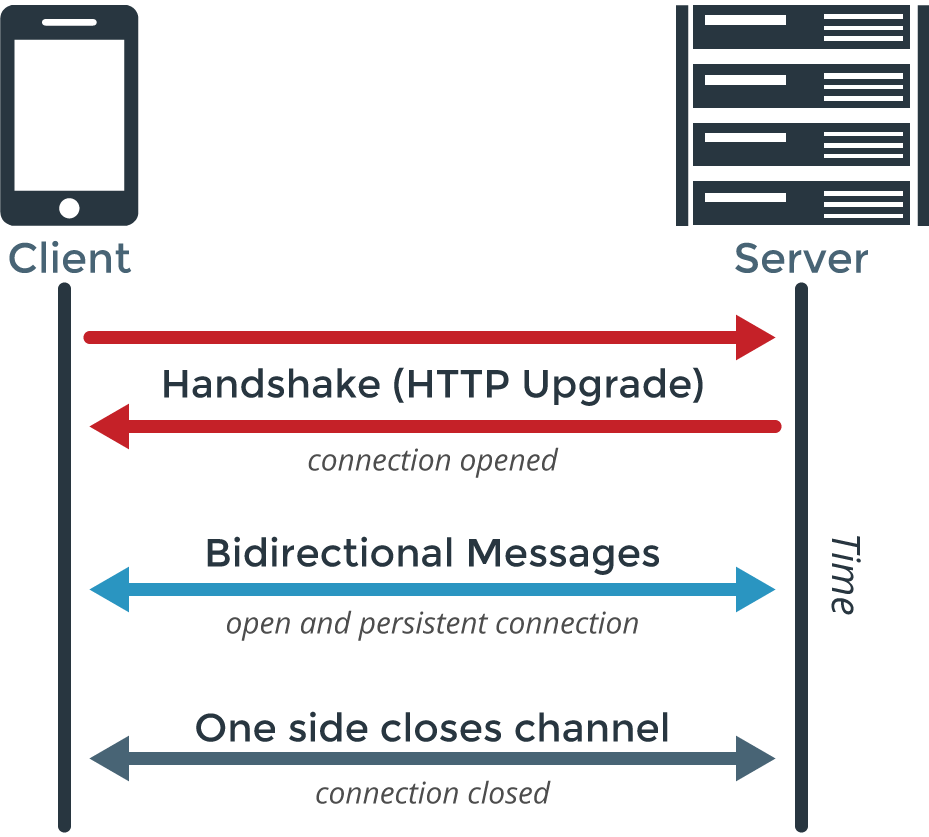
\includegraphics[keepaspectratio = true, totalheight=0.5\textheight]{figuras/ws_diagrama.png}
				\end{figure}
 		\end{frame}

\section{Demostraci\'on}
		\begin{frame}
			\frametitle{Demostraci\'on}
			\vfill
			M\'as informaci\'on y c\'odigos fuente en:
			\url{https://github.com/markopesevski/SDAV_mini-projecte}
			\vfill
 		\end{frame}

%------------------------------------------------

\section*{}
\begin{frame}[plain]
	\addtocounter{framenumber}{-1}

	\begin{center}
		{\Huge{Gracias por\\vuestra atenci\'on}}
	\end{center}
	\begin{center}
		{\large{?`Dudas? ?`Comentarios?}}
	\end{center}
\end{frame}

%----------------------------------------------------------------------------------------

\end{document}
